\section{Experiment with Pozyx}
In order to determine the accuracy of the Pozyx tags we conducted an experiment.
The primary goal of the experiment was to test the accuracy, but a secondary goal of the experiment was to determine the frequencies of updates for each tag.
\\\\
According to research regarding latency in VR \cite{WaltemateThomas2016Tiol} and interactive systems \cite{10.1145/169059.169431} the number of movement errors increase as the latency increases.
According to experiments with VR, the motor performance and sense of body ownership start to decrease at latencies above 75 ms.
This means that the optimal results from these experiments would indicate that the Pozyx system is able to give a refresh rate which allows the system to operate with a latency of less than 75 ms between their physical movement and the in-game reflection of this movement.

\subsection{Setup}
The tags were set to transmit with the highest bitrate with the longest preamble length and with the ranging mode set to precise\cite{pozyx-Performance}.
According to the documentation these values lower the tags update rate to about 9hz which is then divided by the amount of tags used in the system as described in \ref{pozyx:TWR}.
Because the main goal of the experiment was to test the accuracy we decided to use these setting to gives the most accurate positioning.
We can then change the settings at a later point to get try and get the update rate to a level where the latency for the users are acceptable.
The experiment was setup as shown on \autoref{fig:experiment-setup}. 
The experiment was conducted indoors on our campus in the building Novi 9. 
The anchors \texttt{0x632b} and \texttt{0x676e} were mounted on a wall 240 centimeters apart, and the remaining anchors \texttt{0x6738} and \texttt{0x676c} were mounted on a bulletin board.
The number of centimeters accompanying the hexadecimal number of each anchor is the height at which the anchor was mounted during the experiment.
Different heights were chosen as Pozyx documentation suggests that not all anchors should have the same height \cite{pozyx-AnchorHeights}.
The reason for this is the principle of geometric dilution of precision(GDOP), which can cause the error on range measurements to be amplified.

\begin{figure}[H]
    \centering
    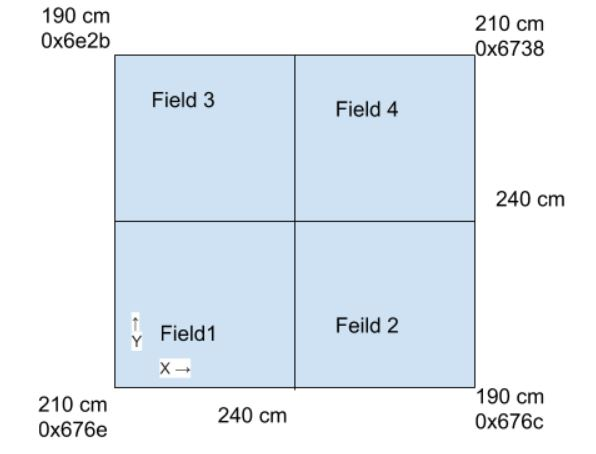
\includegraphics[width=0.6\linewidth]{experiment-setup.JPG}
    \caption{The setup of the experiment with the anchors and the height at which they were placed in the corners.}
    \label{fig:experiment-setup}
\end{figure}
\noindent
The fields were created by a blackboard on which lines were drawn every 10 centimeters to know the actual position as seen on \autoref{fig:experiment-blackboard}.
This blackboard was moved intermittently to act as respectively field 1, field 2, field 3 and field 4.

\begin{figure}[H]
    \centering
    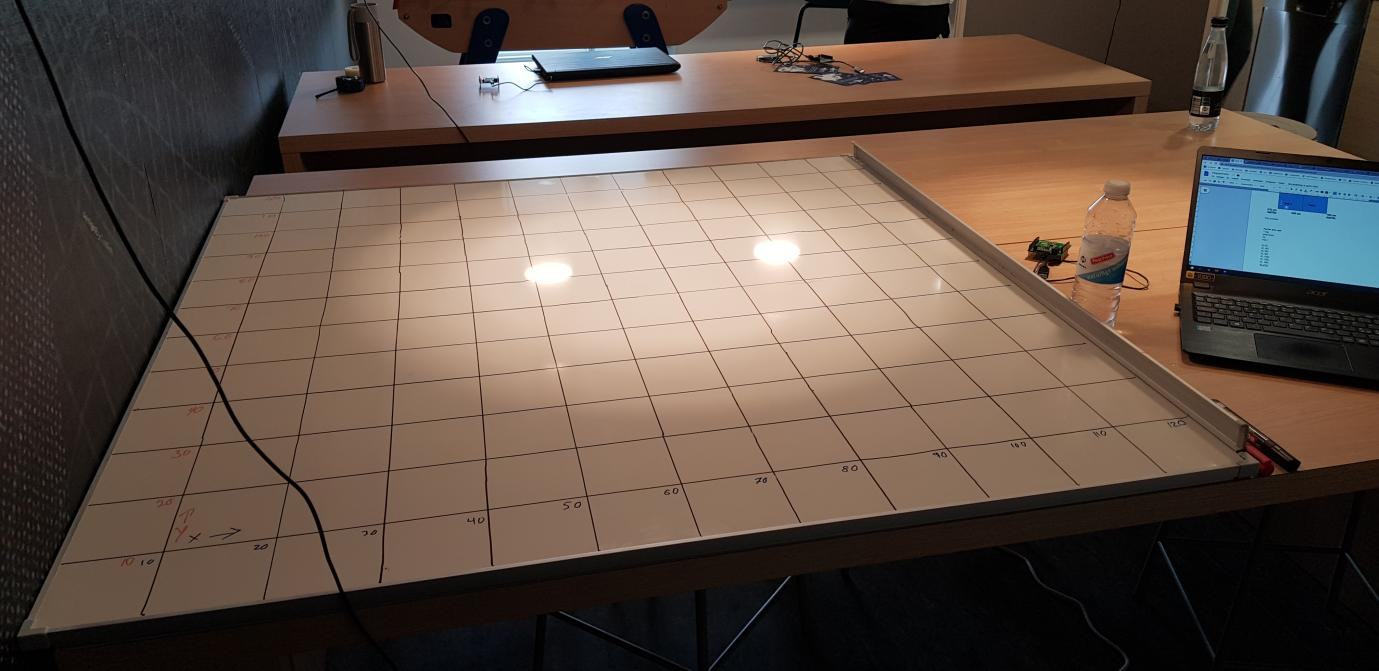
\includegraphics[width=0.8\linewidth]{experiment-blackboard.png}
    \caption{The blackboard with the drawn positions.}
    \label{fig:experiment-blackboard}
\end{figure}
\noindent
The procedure for the experiment was based on this blackboard.
The blackboard would be placed in one of the fields defined in \autoref{fig:experiment-setup}, and we would then place the tags in certain positions on the board and record the accuracy with with the position was reported.
The tags would be placed in a position, remain there for five seconds, then be moved to the next position over the next five seconds and remain in this position for five seconds before being moved again.
This procedure was repeated until a satisfactory number of measurements had been made.
Once one field had been tested, we moved the blackboard to the next field and repeated the setup.
 
\subsection{Work on the data}
In \autoref{app:experiment} the data for the experiment can be seen.
For each test we calculated the average grid, and found the min and max values for \texttt{x}, \texttt{y} and \texttt{z}.
We also calculated the average deviation from the actual grid to the average grid to get a better view of the deviation.
The min and max values were noted, as we might need to take them into account. 
The \texttt{z} values were very inconsistent throughout the entire test, and due to this and the z-axis being largely irrelevant to the game, we have chosen not to analyze them.

\subsubsection{Precision with 1 tag} 
The average of all deviations is 10.54 cm.
There were spikes where the max and min values spiked a lot.
For \texttt{(30, 60)} the minimum $x$ value was -33.3, which is a deviation of around 60 cm and for \texttt{(120, 0)} the minimum $y$ value was -54.5 cm, which is also 54.5 cm away from the actual data point.
There are more cases where the deviation of a single data point is far away. 

\subsubsection{Precision with 3 tag}
For this part of the experiment we tested the accuracy with 3 tags. 

\paragraph{Tag 26467}
The overall average deviation for this tag was 11.2 cm.
There was, however, a large deviation at \texttt{140, 90} and \texttt{(140, 120)} with 20.63 and 20.46 cm.
The min and max values for $x$ and $y$ were good, and there were never any larger spikes from the actual data point than around 25 cm.

\paragraph{Tag 26895}
The overall average deviation for this tag was 6.31 cm.
The average deviation was more accurate than expected for this tag.
For this tag there were also no spikes larger than around 20 cm for the $x$ and $y$ values.

\paragraph{Tag 24622}
The overall average deviation for this tag was 17.41 cm.
The first three points we tested seemed fairly accurate, however the grid \texttt{(220, 90)} and \texttt{(220, 120)} had a large deviation of 37.53 cm and 24.4 cm respectively.
The min and max values for $x$ and $y$ were greater in this than the previous, with around 40 cm deviations.

\subsubsection{Precision with 5 tag}
For this experiment we have also noted how many data points were sent in the 5 second intervals, as well as the average deviation.

\paragraph{Tag 24622}
The average deviation for this tag was 8.42 cm and the average amount of data points every 5 seconds was around 4.28 data points.
However, at \texttt{(180, 120)} we only received 1 data point.
The min and max values of $x$ and $y$ were lower than 25 cm.

\paragraph{Tag 26467}
For this tag the average deviation was 11.20 cm and the average amount of data points was 3.28.
At \texttt{140, 40} there was only one update, and at \texttt{140, 80} there were only 2 updates every 5 seconds.
The max \texttt{x} value was around 30 cm away from the actual data point, but otherwise they did not spiked larger than that.

\paragraph{Tag 26895}
Tag 26895 had an average deviation of 14.78 cm. 
The deviation was higher than the two previous, however there was an average update rate of 9.57, which is more than twice as high as the two previous tags.
The min and max values for min \texttt{y} and max \texttt{y} deviated at \texttt{(160, 20)}, where the min value for x was -28 cm, and max value was 49.4 cm.

\paragraph{Tag 26901}
The average deviation of tag 26901 was 8.56 cm, and it sent an average of 10 data points every 5 seconds.
This tag was quite stable, as there were 10 data points every 5 seconds almost every time, and the average deviation never spiked higher than 12 cm.
Around \texttt{(220, 100)} the min $y$ value was 51.3 cm, which is quite far away from the actual position.
There were a few instances of large gaps between min and max values and actual grid.

\paragraph{Tag 27001}
The average deviation of this tag is 9.61 and the average amount of data points every 5 seconds was 5.57.
This was also quite consistent with the average deviation. 
The max values for $x$ and $y$ was also quite consistent and there were no large deviations.
The min and max deviation of the $x$ coordinate was quite accurate with a largest distance of around 20 cm, but mostly less than 10 cm.
The $y$ coordinate fluctuated more, but was still less than 25 cm.

\subsection{Possible influences on the test}
One thing that could have affected the tags is that we used a blackboard as a measure for positions. 
As there is metal in the blackboard this could have affected the precision on the tags.
Metals are conductors, which can lead to the signal having less power and reduced range, and the signal might spend extra time trying to get through the metal.
Since Pozyx positioning relies on calculating the time of flight, having the signal spend extra time travelling reduces accuracy \cite{pozyx-UWBObstacles}. 
\\\\
During the test with 1 tag, the 0 value of the $x$ coordinate coincided with the wall. 
This could have been an influence on the positing result in that it could increase uncertainty, as it was difficult to center the tag over the x coordinate since the coordinate collided with the wall.
\\\\
While the experiment was running the tags could throw errors instead of giving a position if something went wrong.
Mainly during the multi tag tests some tags would report back with errors such as unable to get firmware version, flash memory corrupted or an error message saying there was no error.
At that point of the experiment it was not clear whether it was a hardware error with some of the tags or if it was code related.
The tags would throw these errors randomly and then report back their position like normal at the next update.
This resulted in some of the tags having periods of update rates of less than 0.2 Hz.
It was decided that further investigation into this issue should be conducted at a later point.

\subsection{Conclusion on the experiment}
Our conclusion of this experiment is that the precision is satisfactory, but we need to do something about the update rate as that does not meet the standards of the refresh rate needed.
\\\\
We also need to consider the spikes in the coordinates, such that the user does not jump around on screen, even though the user might not be moving.
\\\\
It also seemed like some tags was not able to send as many data points as others. This was also due to getting errors from some of the tags.
This is something that should be investigated.
